\textbf{Exemplary latex documents:}
\begin{itemize}
    \item \href{https://v2.overleaf.com/read/vdvhrkdzyvqp}{Network Exercise 8} with Henning and Sophie where we mostly did graphs with the \texttt{tikz} package
    \item \href{https://v2.overleaf.com/read/sydtwzsdgqjx}{My SMMD homework} where I included code in the document
\end{itemize}

\textbf{From Funk's mail:}\\
- intro to the paper ("2 pages": research question, data \& method, results + errors you discovered \& ideas to extend the study, if any)\\
- section on data simulation (explain how you did it, what were challenges and your solutions, open questions?)\\
- section on model estimation (explain how you did it, results, optional: vary the data generation process and describe the impact on the model estimation)\\
- Overall the final report "could" have 3000-4000 words (without source code and tables), but you are free to do what suits your purpose; be innovative;-)

Residuals
\begin{figure}
    \centering
    \includegraphics[scale=0.4]{CTR}
    \caption{An overview to the components of CTR}
    \label{fig:CTR}
\end{figure}

\begin{figure}
    \centering
    \includegraphics[scale = 0.45]{AdPos}
    \caption{An example for a endogenous variable, Ad Position}
    \label{fig:AdPos}
\end{figure}

The overall hierarchical model has been summarized including the distributions used. %like in the Kruschke book - up to discussion what exactly it looks like.

\begin{figure}
    \begin{subfigure}{0.6\textwidth}
        \includegraphics[width=0.95\linewidth]{FullModel} 
        \caption{Full model}
        \label{fig:subFullModel}
    \end{subfigure}
    \begin{subfigure}{0.39\textwidth}
        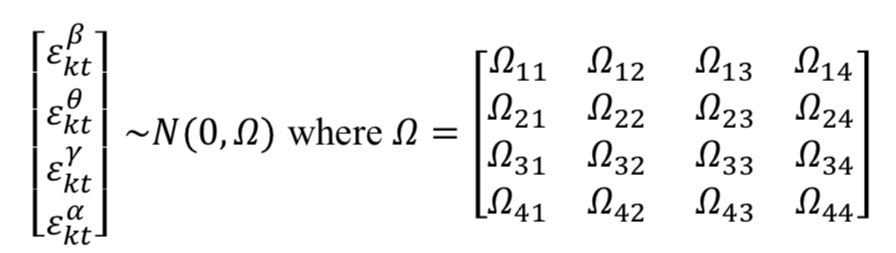
\includegraphics[width=0.95\linewidth]{omega}
        \caption{$\Omega$ as the standard error to the estimates of the errors $\epsilon$}
        \label{fig:subomega}
    \end{subfigure}
    \caption{E.g. to estimate $\epsilon^{\theta}_{kt}$ (the lowest "leaf" of the left-hand tree marked in green), the matrix of standard errors $\Omega$ has to be estimated first. Expression from equation 7, p. 26.}
    \label{fig:Omegacomparison}
\end{figure}

- multivariate regression stemming from zellner, taken from the bayesian statistics in marketing book, p. 31.\\


In general, the paper provided the group with a good example of how a hierarchical model can be applied to a particular setting. Both data simulation and model estimation offered an invaluable learning and coding experience, and helped to understand the processes from within. Moreover, the topic of online advertisement performance evaluation appealed to the group members, combining practical applicability and an interesting insight into a hot topic for data science professionals with scientific character of a research paper. Nevertheless, several drawbacks of the examined paper hindered the work and possibly its outcomes.\\

The coefficients used in the paper model are referred to by both Greek letters and the contextual names, explaining the idea behind the said coefficients, such as \textit{Adpos} or \textit{SponsoredComp}; however, the estimates are not clearly defined. Due to that it's not exactly clear how each particular estimate comes into the model.\\

While these differences are neither unexpected, nor critical for the model, they show the limitation the group could face if they were to try to replicate the same field experiment hoping to get the very same results just because the group managed to replicate the model itself, and thus disregarding the new ad positioning.\\ 
As mentioned above, these disadvantages still don't undermine the learning potential of the examined paper.


Notes:\\
- a table and graphs for estimate comparison\\


%[...] The results somewhat match the authors' results in table 4, Figure \ref{fig:table4}. Again, it is not clear what exactly these values stand for, but the group decided to treat the table as estimates for the $\theta$ coefficients in the case of CTR and for the $\beta$ coefficients in the case of the conversion rate. As an example, $\theta^k_3$ as the bias of $sponsoredComp_{kt}$$ has been listed as "Sponsored Competition" in this table.\\

%%%% They somehow also used a data augmentation approach.
% https://medium.com/nanonets/how-to-use-deep-learning-when-you-have-limited-data-part-2-data-augmentation-c26971dc8ced
% this we'll have to do: compare our thetas from calc_weights to the paper (sd given)